%%%%%%%%%%%%%%%%%%%%%%%%%%%%%%%%%%%%%%%%%%%%%%%%%%%%%%%%%%%%%%%%%%%%%%%%%%%%%%%%%%%%
% Document data
%%%%%%%%%%%%%%%%%%%%%%%%%%%%%%%%%%%%%%%%%%%%%%%%%%%%%%%%%%%%%%%%%%%%%%%%%%%%%%%%%%%%
\documentclass[12pt]{article} %report allows for chapters
%%%%%%%%%%%%%%%%%%%%%%%%%%%%%%%%%%%%%%%%%%%%%%%%%%%%%%%%%%%%%%%%%%%%%%%%%%%%%%%%%%%%
\usepackage{preamble}
\newcommand{\grad}{\boldsymbol{\vec{\nabla}}}
\newcommand{\curvegamma}{\boldsymbol{\vec{\gamma}}}
\newcommand{\tangentgamma}{\boldsymbol{\dot{\vec{\gamma}}}}
\newcommand{\normalgamma}{\boldsymbol{\ddot{\vec{\gamma}}}}
\newcommand{\vecfieldE}{\boldsymbol{\vec{E}}}
\newcommand{\rhat}{\boldsymbol{\hat{r}}}
\newcommand{\thetahat}{\boldsymbol{\hat{\theta}}}
\newcommand{\phihat}{\boldsymbol{\hat{\phi}}}
\newcommand{\rhohat}{\boldsymbol{\hat{\rho}}}
\newcommand{\unitvec}{\boldsymbol{\hat{n}}}
\newcommand{\vecfieldB}{\boldsymbol{\vec{B}}}
\newcommand{\vecfieldJ}{\boldsymbol{\vec{J}}}
\newcommand{\vecfieldF}{\boldsymbol{\vec{F}}}



\begin{document}

\begin{center}
   \textsc{\large MATH 272, Homework 7, \emph{Solutions}}\\
   \textsc{Due March 31$^\textrm{st}$}
\end{center}
\vspace{.5cm}

\begin{problem}
    Plot each of the following vector fields.
    \begin{enumerate}[(a)]
        \item $\rhohat = \frac{x}{\sqrt{x^2+y^2}}\xhat + \frac{y}{\sqrt{x^2+y^2}}\yhat$.
        \item $\thetahat = \frac{-y}{\sqrt{x^2+y^2}}\xhat + \frac{x}{\sqrt{x^2+y^2}}\yhat$.
        \item $\zhat$.
    \end{enumerate}
\end{problem}
\begin{solution} Here are the plots for these three fields.

\begin{enumerate}[(a)]
    \item The plot for $\rhohat$.
    \begin{figure}[H]
        \centering
        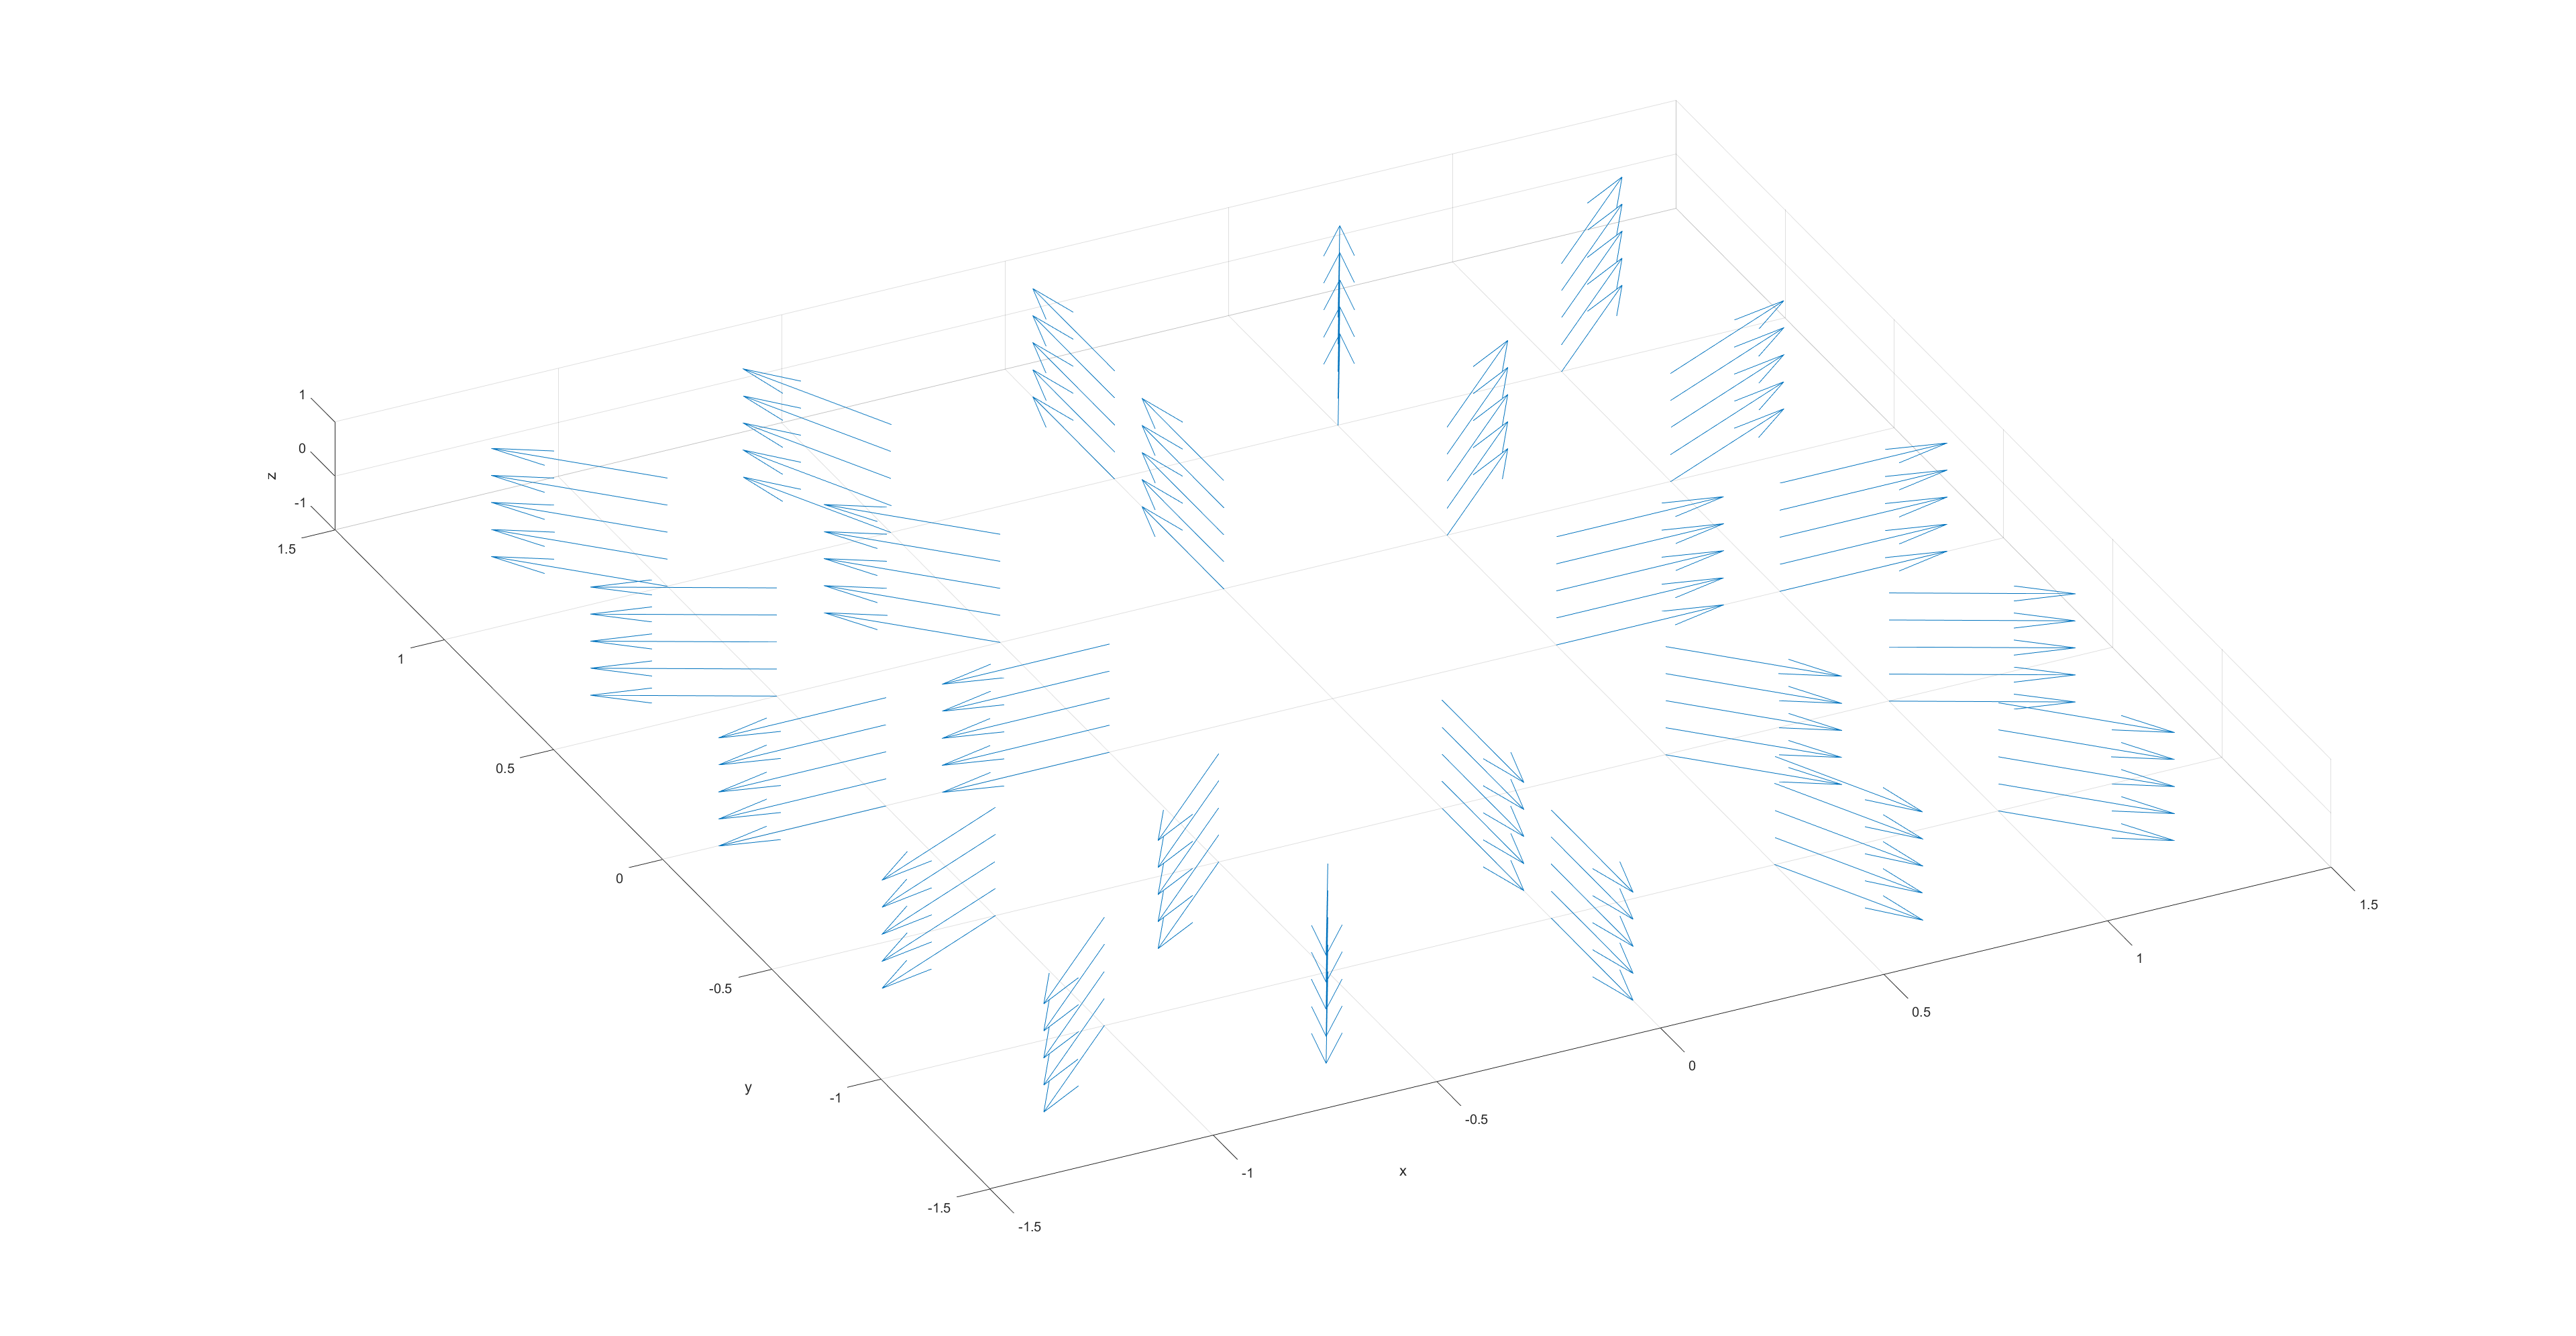
\includegraphics[width=\textwidth]{rho_hat.png}
    \end{figure}
    \item The plot for $\thetahat$.
    \begin{figure}[H]
        \centering
        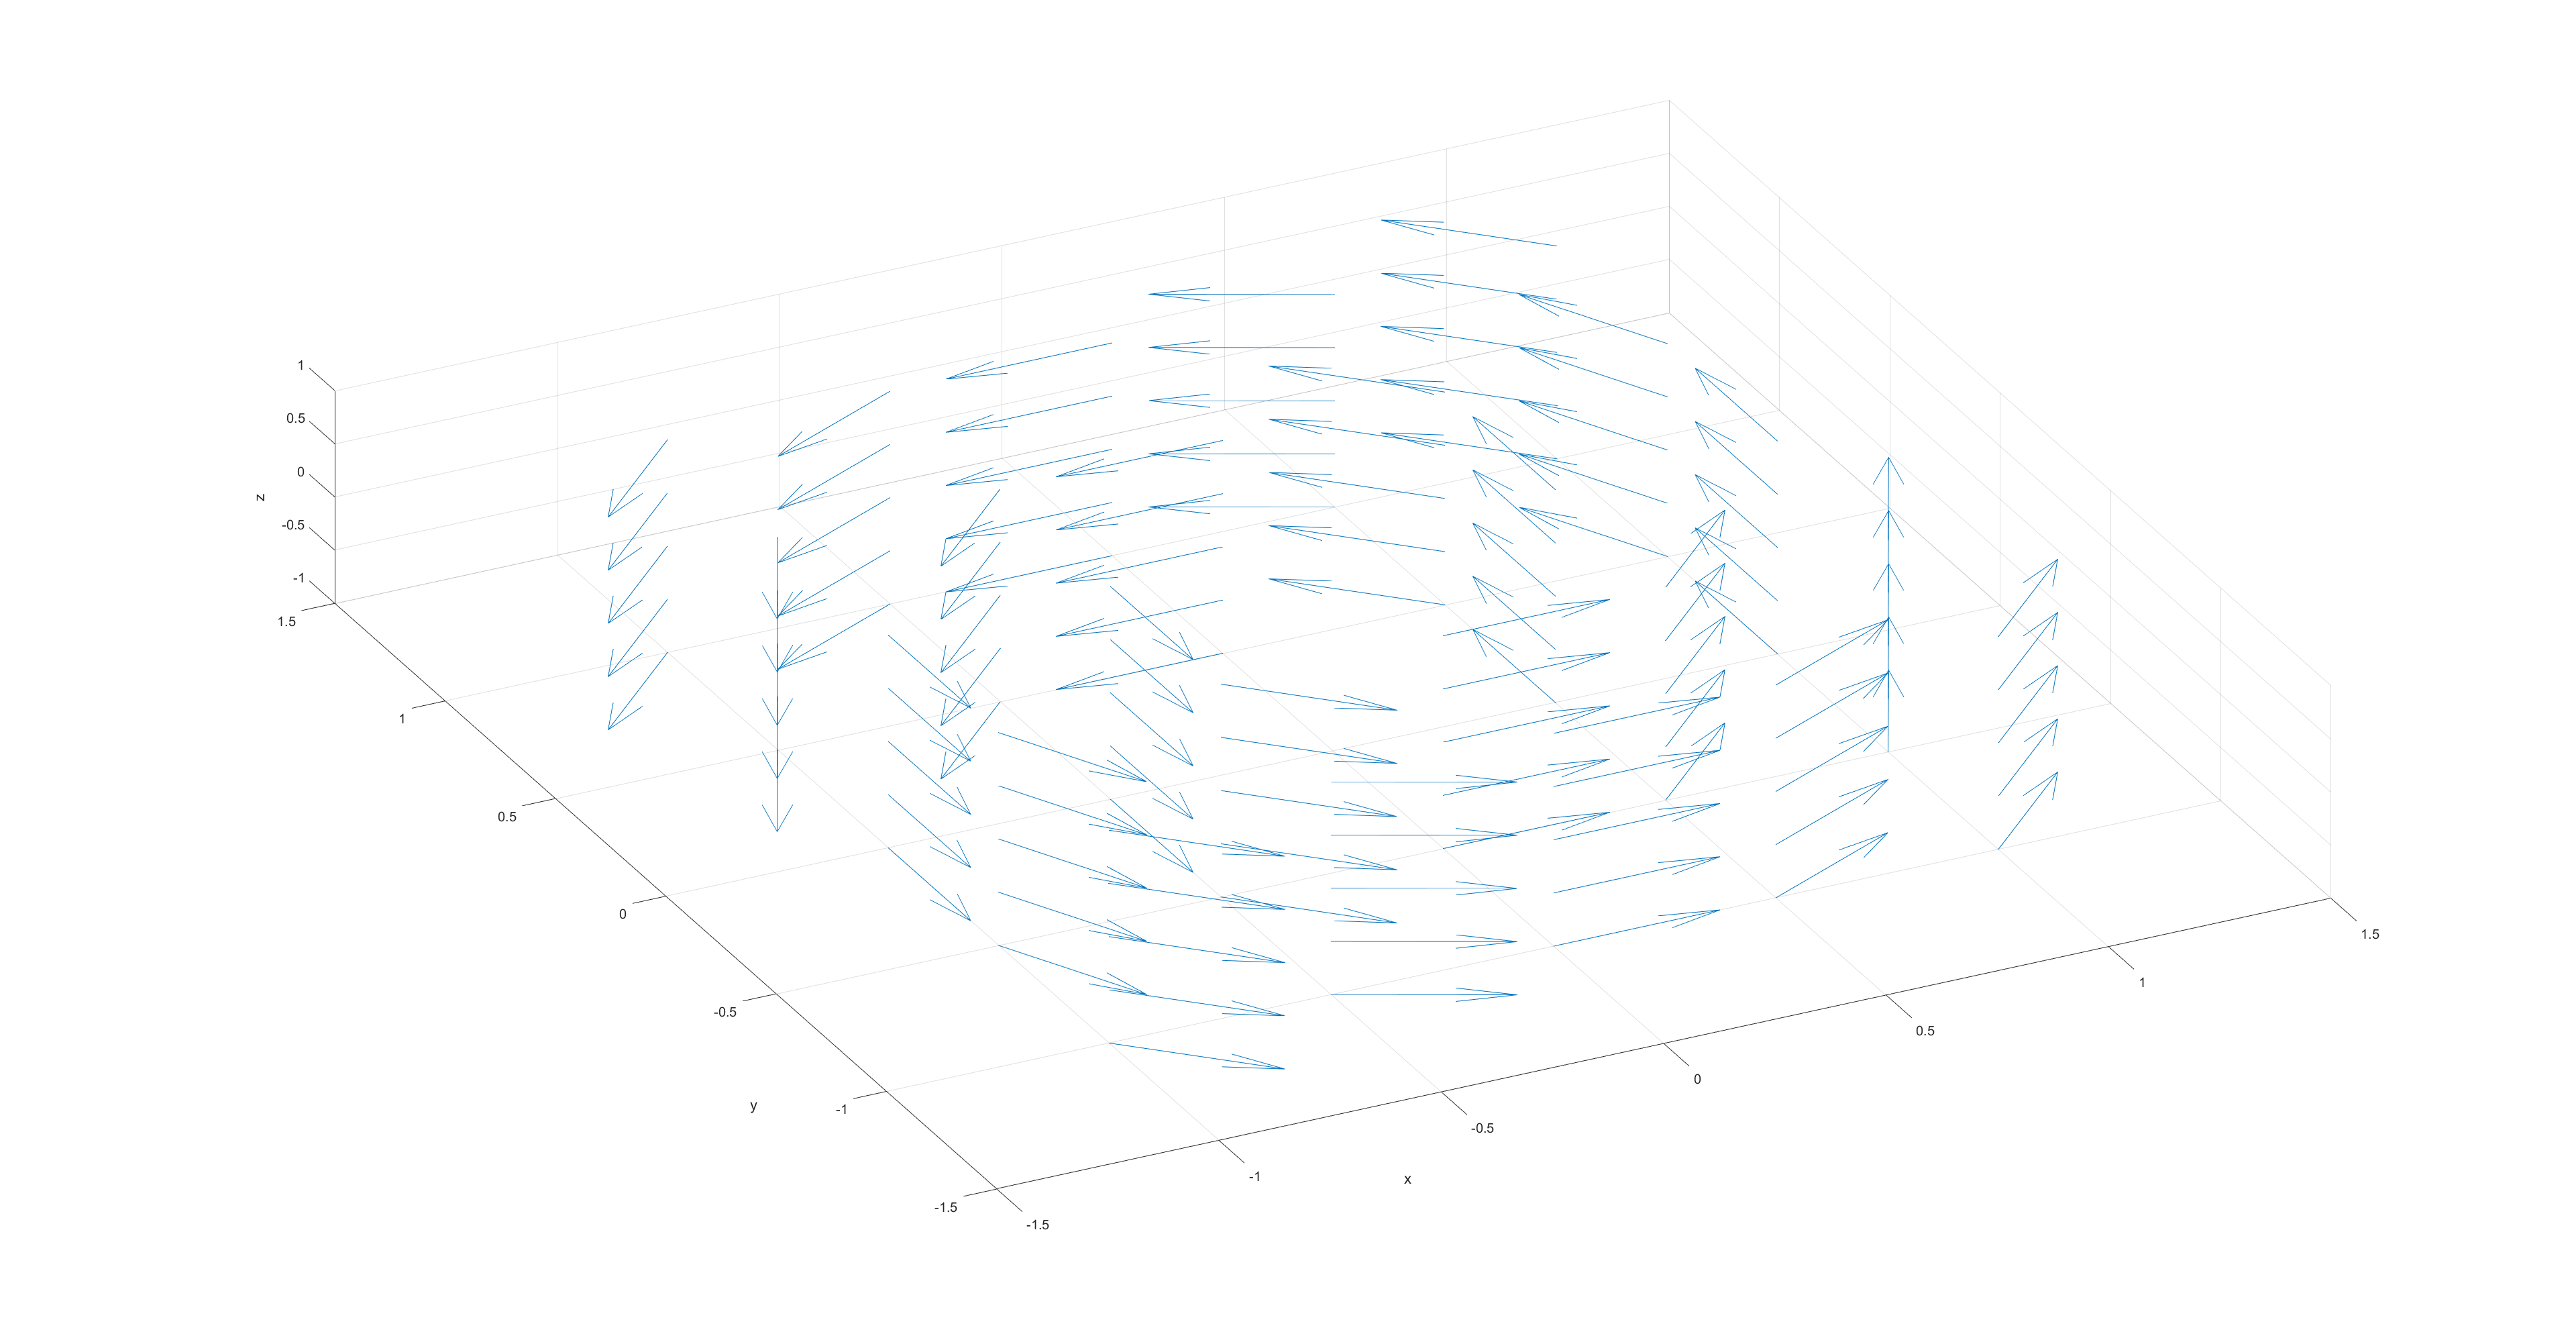
\includegraphics[width=\textwidth]{theta_hat.png}
    \end{figure}
    \item The plot for $\zhat$.
    \begin{figure}[H]
        \centering
        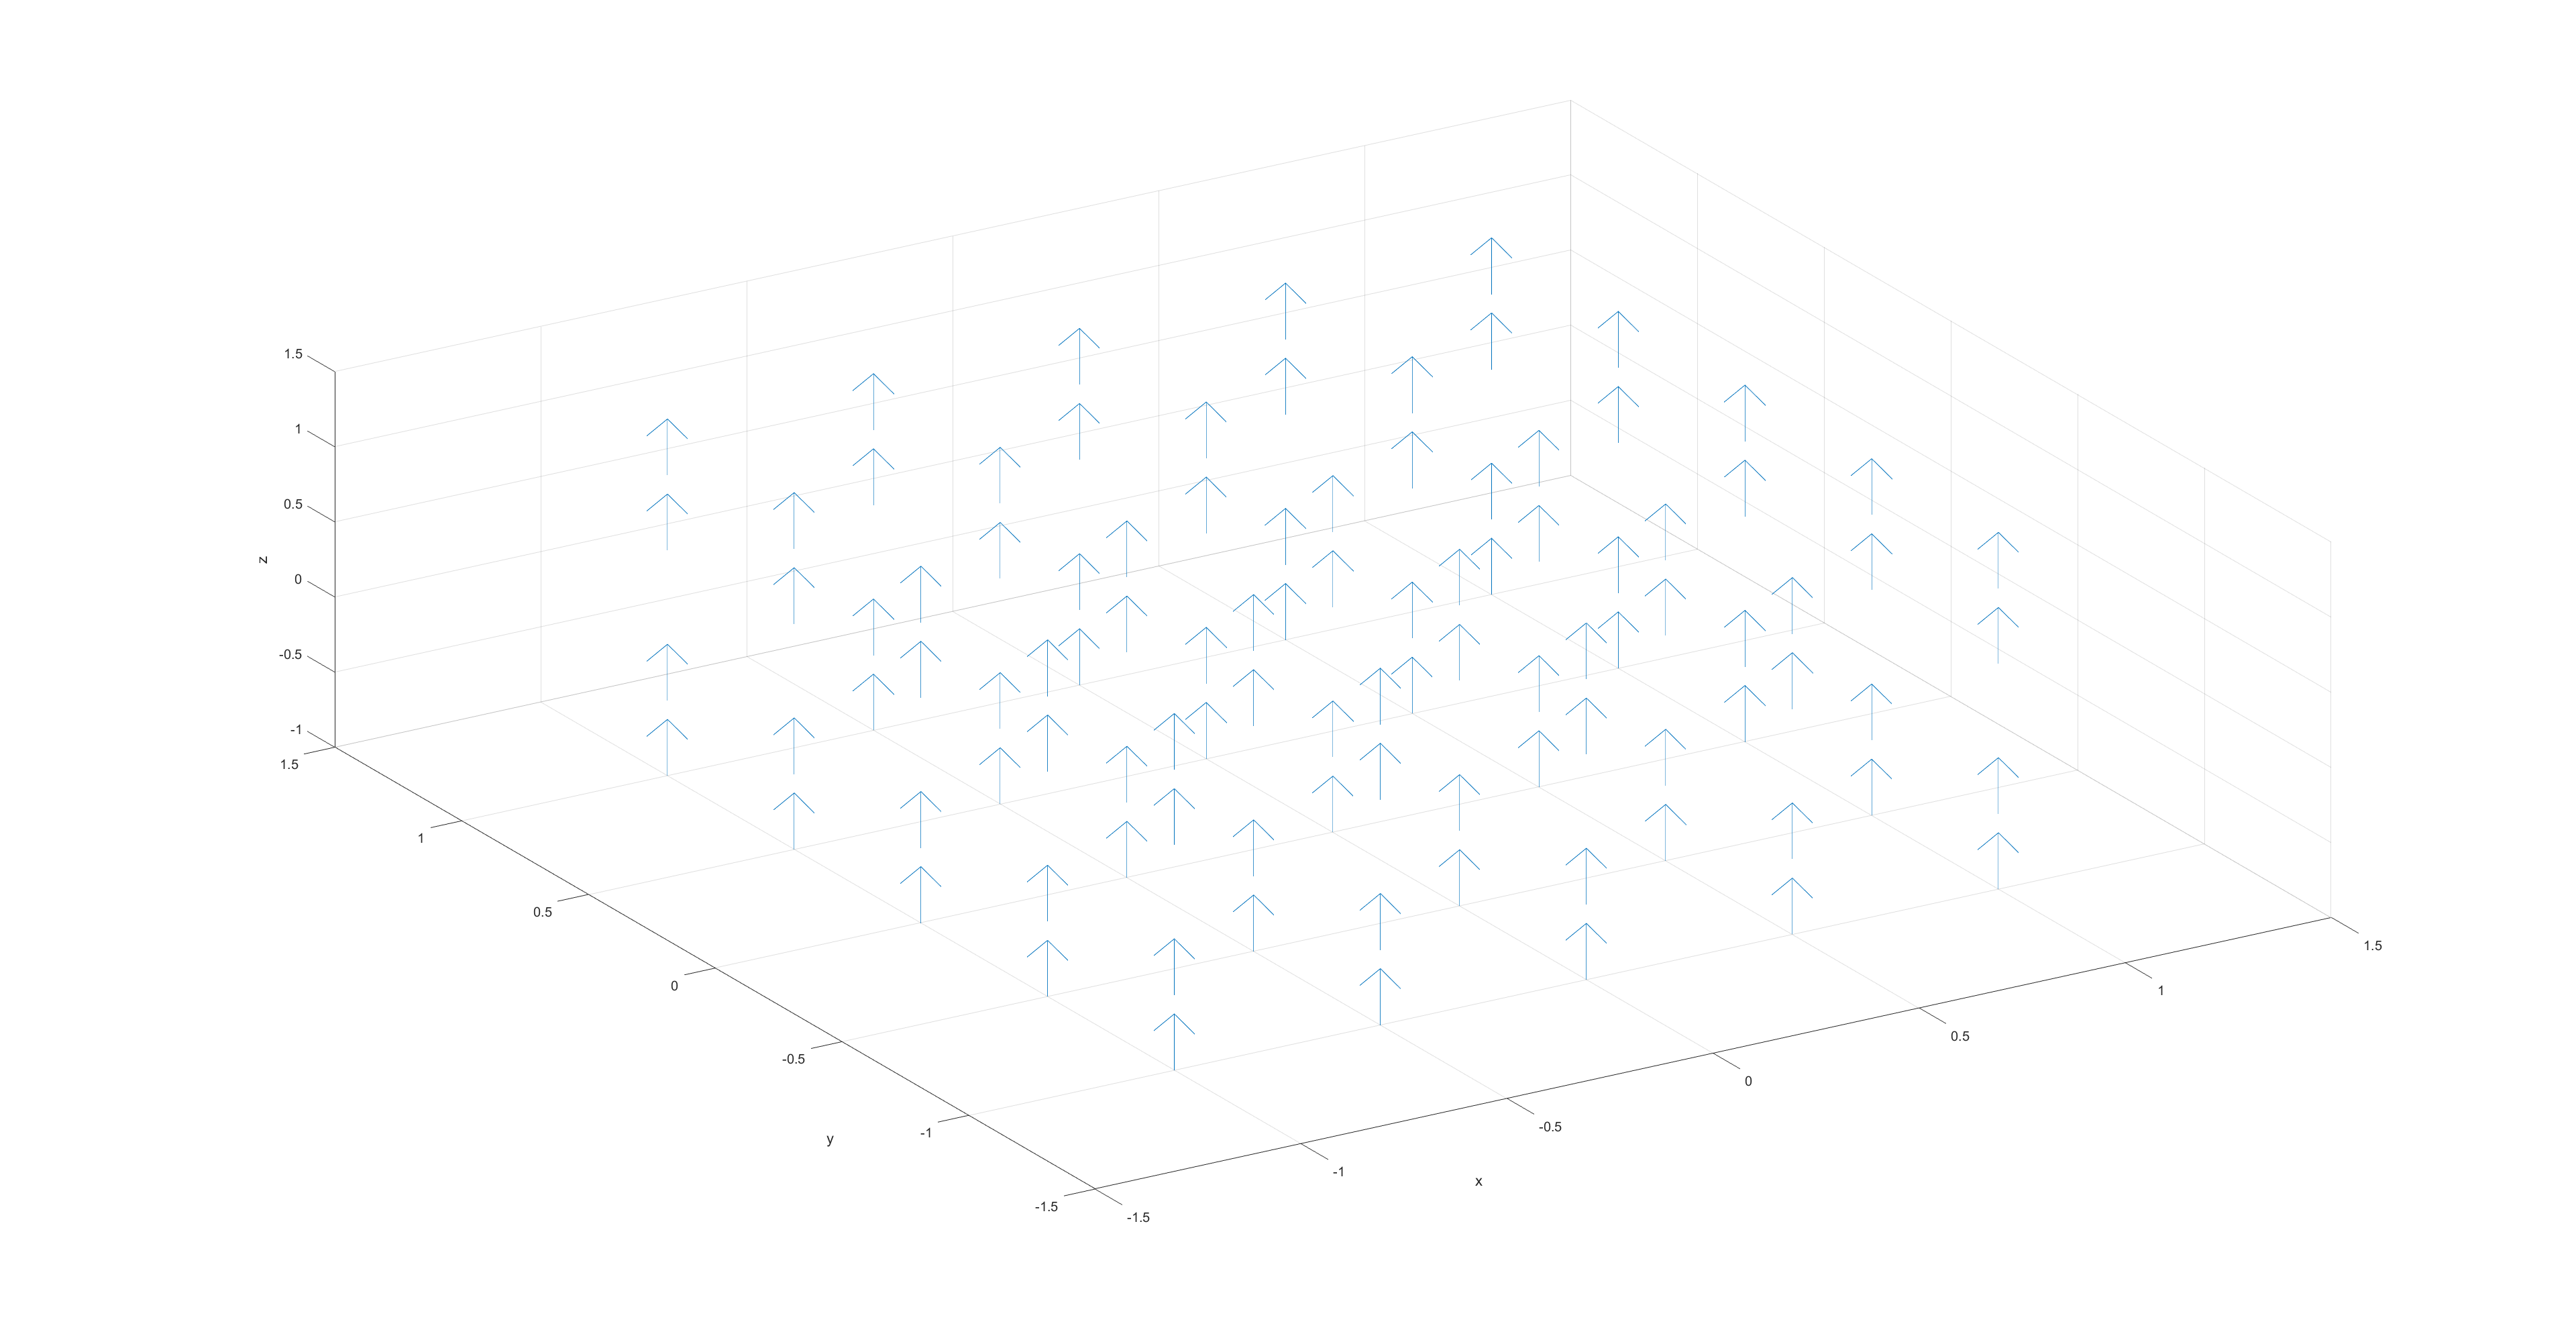
\includegraphics[width=\textwidth]{z_hat.png}
    \end{figure}        
\end{enumerate}

\end{solution}

\newpage
\begin{problem}
Consider the following vector field
\[
\vecfieldB = -\frac{y}{2}\xhat + \frac{x}{2}\yhat.
\]
Here, $\vecfieldB$ denotes the magnetic field. It may be helpful to plot the fields in this problem.
\begin{enumerate}[(a)]
    \item Show that $\grad \times \vecfieldB = \vecfieldJ$ (Amp\'ere's law) where 
    \[
    \vecfieldJ = \zhat.
    \]
    This vector field $\vecfieldJ$ represents the electric current (moving charges) in space. One could argue that the current creates the magnetic field via Amp\'ere's law.
    \item Magnetic fields induce a force $\vecfieldF$ on charged particles by the Lorentz force
    \[
    \vecfieldF = \tangentgamma \times \vecfieldB = \normalgamma
    \]
    Where $\tangentgamma$ is the velocity of the particle (where we have chosen a mass $m=1$ and charge $q=1$).  Let us do the following.
    \begin{itemize}
        \item Assume that $\tangentgamma = \xhat$, what is the force on the particle?
        \item Repeat the previous step for $\tangentgamma=\yhat$ and $\tangentgamma=\zhat$. 
        \item Compare and contrast the forces you found.
    \end{itemize}
    \item Can you argue why applying a magnetic field to a molecule may cause it to heat up? Can you compare this idea with your home microwave? (Please don't put anything dangerous in your microwave due to this discovery!)
\end{enumerate}
\end{problem}
\begin{solution}~
\begin{enumerate}[(a)]
    \item We have
    \begin{align*}
        \begin{pmatrix} \frac{\partial}{\partial x} \\ \frac{\partial}{\partial y} \\ \frac{\partial}{\partial z} \end{pmatrix} \times \begin{pmatrix} \frac{-y}{2} \\ \frac{x}{2} \\ 0 \end{pmatrix} &= \begin{pmatrix} 0 \\ 0 \\   \frac{\partial}{\partial x} \frac{x}{2} - \frac{\partial}{\partial y} \frac{-y}{2} \end{pmatrix} \\
                &= \begin{pmatrix} 0 \\ 0 \\ 1 \end{pmatrix}\\
                &= \zhat.
    \end{align*}
    \item We will look at the case for the three different tangent vectors.
    \begin{itemize} 
        \item If $\tangentgamma = \xhat$, then
        \[
        \tangentgamma \times \vecfieldB = \frac{x}{2}\zhat.
        \]
        \item If $\tangentgamma = \yhat$, then
        \[
        \tangentgamma \times \vecfieldB = \frac{y}{2} \zhat.
        \]
        \item Finally, if $\tangentgamma =\zhat$, then
        \[
        \tangentgamma \times \vecfieldB = -\frac{y}{2}\yhat -\frac{x}{2}\xhat.
        \]
    \end{itemize}
    Note that if $\tangentgamma$ is in the $x$- or $y$-direction, we get a force that is aligned in the $z$-direction.  When $\tangentgamma$ is in the $z$-direction, then the forces are in the $x$- and $y$-direction. Moreover, the forces that align in the $z$-direction will cause the particle to move away indefinitely in the $z$-direction whereas when the force is in the $x$- or $y$-direction, we will have a force that causes the particle to oscillate.
    
    \item If we apply a magnetic field to charged particles, the particles undergo forces. By giving particles more energy of motion, we are heating them up.  If we apply the correct kind of magnetic field, it is conceivable that we would simply causes a particle to vibrate with more intensity.
\end{enumerate}
\end{solution}

\newpage
\begin{problem}
Let us see some of the usefulness of cylindrical coordinates.
\begin{enumerate}[(a)]
    \item Using the fact that $\thetahat = \frac{-y}{\sqrt{x^2+y^2}}\xhat + \frac{x}{\sqrt{x^2+y^2}}\yhat$, convert the magnetic field from Problem 2 into Cylindrical coordinates (i.e., only a function of $\rho$, $\theta$, $z$, and $\rhohat$, $\thetahat$, and $\zhat$).  
        \item Parameterize a curve $\curvegamma(t)$ that traces out the unit circle in the $xy$-plane in cylindrical coordinates.
        \item What is the tangent vector $\tangentgamma(t)$ in terms of $\rhohat$, $\thetahat$, and $\zhat$?
        \item Compute the following integral using cylindrical coordinates that we have found:
        \[
        \int_{\curvegamma} \vecfieldB \cdot d\curvegamma
        \]
        \item Using cylindrical coordinates, compare your result with
        \[
        \iint_\Sigma \left(\grad \times \vecfieldB\right) \cdot \unitvec d\Sigma,
        \]
        where $\Sigma$ is the unit disk.
\end{enumerate}
\end{problem}
\begin{solution}~
\begin{enumerate}[(a)]
    \item We have that
    \[
    \vecfieldB = -\frac{y}{2} \xhat + \frac{x}{2}\yhat.
    \]
    Then, note that we have
    \begin{align*}
        \vecfieldB &= \frac{1}{2}\sqrt{x^2+y^2} \left( \frac{-y}{\sqrt{x^2+y^2}} \xhat + \frac{x}{\sqrt{x^2+y^2}} \right)\\
        &=\frac{1}{2} \sqrt{x^2+y^2} \thetahat.
    \end{align*}
    Finally, we have that $\rho = \sqrt{x^2+y^2}$ and hence
    \[
    \vecfieldB = \frac{\rho}{2} \thetahat.
    \]
    \item It suffices to find functions $\rho(t)$, $\theta(t)$, and $z(t)$ to create the curve
    \[
    \curvegamma(t) = \rho(t) \rhohat + \theta(t) \thetahat + z(t) \zhat.
    \]
    Note that for a circle centered along the $z$-axis, we have that $\rho$ is constant and in this case since we are considering the unit circle, we have $\rho(t)=1$.  Similarly, we want the circle to lie in the $xy$-plane where $z=0$, hence we must have $z(t)=0$.  Finally, we must trace the whole unit circle so we must have $\theta$ cover all of $[0,2\pi)$. One choice is to have $\theta(t)=t$ for $t\in[0,2\pi)$, but there are many other options! Using these choices, we have
    \[
    \curvegamma(t) = \rhohat + t \thetahat.
    \]
    \item Then, we have the tangent vector $\tangentgamma = \frac{d\curvegamma}{dt}$ and thus
    \[
    \tangentgamma(t) = \thetahat.
    \]
    \item Note that from the above work we have
    \[
    d \curvegamma = \tangentgamma dt = \thetahat dt.
    \]
    Thus, 
    \[
    \vecfieldB \cdot \tangentgamma = \frac{\rho}{2}.
    \]
    This gives us that
    \begin{align*}
        \int_{\curvegamma} \vecfieldB \cdot d\curvegamma &= \int_0^{2\pi} \frac{\rho(t)}{2}dt\\
        &=\int_0^{2\pi} \frac{1}{2} dt\\
        &= \pi.
    \end{align*}
    Above, we can note that $\rho(t)=1$ since we are integrating along the unit circle in the $xy$-plane.
    \item We had computed $\grad \times \vecfieldB = \zhat$ earlier.  Then, the unit disk has the normal vector $\unitvec=\zhat$ and thus
    \[
    \left( \grad \times \vecfieldB \right) \cdot \unitvec = 1.
    \]
    Now we have
    \[
    \iint_{\Sigma} \left( \grad \times \vecfieldB \right) \cdot \unitvec d\Sigma = \iint_{\Sigma} d\Sigma,
    \]
    which is equal to the area of the unit disk.  So, we don't even need to compute the integral by finding bounds and since we know the area of the unit circle is $\pi$.  It follows that
    \[
    \pi = \iint_{\Sigma} \left( \grad \times \vecfieldB \right) = \int_{\curvegamma} \vecfieldB \cdot d\curvegamma.
    \]
    Indeed, the two integrals are equal (possibly up to a sign depending on your work). 
\end{enumerate}
\end{solution}

\newpage
\begin{problem}
    Convert the following integrals to integrals in cylindrical coordinates. Also, describe the region in which you are integrating over. Do not evaluate the integrals.
    \begin{enumerate}[(a)]
        \item $\displaystyle{\int_{-1}^{1} \int_{-1}^{1} \int_{-\sqrt{1-y^2}}^{\sqrt{1-y^2}} xyz dxdydz}$.
        \item $\displaystyle{\int_0^1 \int_{-z}^z \int_{-\sqrt{z^2-y^2}}^{\sqrt{z^2-y^2}} x^2+y^2+z^2 dxdydz}$.
    \end{enumerate}
\end{problem}
\begin{solution}~
\begin{enumerate}[(a)]
    \item First, let us convert the integrand to cylindrical coordinates. We have
    \[
    xyz = \rho \cos (\theta) \rho \sin(\theta) z = \rho^2 \cos(\theta)\sin(\theta)z.
    \]
    Now, as for the bounds to the integral, we are letting
    \[
    -\sqrt{1-y^2}\leq x \leq \sqrt{1-y^2}.
    \]
    If we square the above equation, we get
    \[
    1-y^2 \leq x^2 \leq 1-y^2,
    \]
    which means that
    \[
    x^2+y^2 =1.
    \]
    This is the implicit equation for the unit circle in the $xy$-plane.  So, if we then let $y$ range from $-1$ to $1$, we must be integrating over the unit disk in the $xy$-plane.  Then, we have $-1\leq z\leq 1$, so it must be that we are integrating over a cylindrical region.  So, to convert the whole integral to cylindrical coordinates, we note that
    \[
    dxdydz = \rho d\rho d\theta dz,
    \]
    and thus
    \[
    \int_{-1}^{1} \int_{-1}^{1} \int_{-\sqrt{1-y^2}}^{\sqrt{1-y^2}} xyz dxdydz = \int_{-1}^1 \int_{0}^{2\pi} \int_{0}^1 \rho^3 \cos(\theta)\sin(\theta)z d\rho d\theta dz.
    \]
    \item The intuition from (a) can help us here. We can note
    \[
    x^2+y^2+z^2 = \rho^2+z^2
    \]
    and as always
    \[
    dx\,dy\,dz = \rho \, d\rho \, d\theta \, dz.
    \]
    The bounds for $x$ and $y$ are similar to (a), except that we have that the radius of the circle depends on $z$ and is not just fixed at 1 since we can repeat the work above to get
    \begin{align*}
        -\sqrt{z^2-y^2}\leq &x \leq \sqrt{z^2-y^2} \\
        \implies ~ x^2&= z^2-y^2 \\
        \implies ~ x^2+y^2-z^2=0,
    \end{align*}
    which is the implicit equation for a double cone. Thus, we have that we are integrating over just a part of this double cone! In cylindrical coordinates, this gives us that $\rho^2=z^2$ and that $z=\pm\rho$. However, we require $0\leq z \leq 0$, so $\rho=z$.  Thus, our integral then becomes
    \[
    \int_0^1 \int_{-z}^z \int_{-\sqrt{z^2-y^2}}^{\sqrt{z^2-y^2}} x^2+y^2+z^2 dx\,dy\,dz = \int_{0}^1 \int_0^{2\pi} \int_{0}^z \left(\rho^2 + z^2 \right) \rho \, d\rho \, d \theta\, dz. 
    \]
    
    \end{enumerate}
\end{solution}

\newpage
\begin{problem}
	In spherical coordinates (either implicitly or explicitly), parameterize the following objects.
	\begin{enumerate}[(a)]
		\item A solid sphere with radius 3.
		\item The surface of an infinite cone with a vertex angle of $\pi/4$.
		\item A latitudinal curve on the unit sphere at the latitude of 30$^\circ$ above the equator.
		\item A solid unit sphere with a cylinder of radius 1/2 removed from the core.
	\end{enumerate}
\end{problem}
 \begin{solution} ~
 \begin{enumerate}[(a)]
    \item In this case, it's easiest to just take $0\leq r \leq 3$, $0\leq \theta < 2\pi$ and $0\leq \phi \leq \pi$.  
    \item Here, we let $\phi=\frac{\pi}{8}$ so that the vertex angle is $\frac{\pi}{4}$.  Then we let $r\in [0,\infty)$ and $\theta \in [0,2\pi)$.
    \item We can write this in spherical coordinates by noting that 30$^\circ$ is $\frac{\pi}{6}$ and that we can get $\phi(t)$ must be constant and indeed 
    \[
    \phi(t) = \frac{\pi}{2}-\frac{\pi}{6}=\frac{\pi}{3}.
    \]
    Then, since the curve is on the unit sphere, it must be that $r(t)=1$ and finally we have freedom to choose $\theta(t)$ so long as $\theta$ runs over the range $[0,2\pi)$. Most easily is to take $\theta(t)=t$ and $t\in [0,2\pi)$ to get the curve
    \[
    \curvegamma(t) = \rhat + t \thetahat +\frac{\pi}{3} \phihat.
    \]
    \item Recall that a cylinder of radius $\frac{1}{2}$ has the equation
    \[
    x^2+y^2=\frac{1}{4}.
    \]
    The unit sphere is given by $r\leq 1$ with $\theta \in [0,2\pi)$ and $\phi \in [0,\pi]$. However, one can see that for this object to be properly parameterized, we need that $r$ depends on $\phi$.  Drawing from a side profile can lead one to find that we must always have the small value for $r$ is
    \[
    r_{\textrm{min}} \sin \phi = \frac{1}{2}
    \]
    Then, it must be that at smallest $\phi = \frac{\pi}{6}$ since when $r=1$ we have $\phi = \arcsin(1/2) = \frac{\pi}{6}$.  So, the description is given by $\phi \in [\pi/6, 5\pi/6]$ with $\frac{1}{2\sin \phi} \leq r \leq 1$ and $\theta \in [0,2\pi)$.
 \end{enumerate}
\end{solution}
\end{document}